\chapter*{Introduction}

Programma:
\begin{itemize}
    \item Teoria dell'Informazione
    \item Teoria della Complessità
    \item Algoritmi su Grafi ecc \dots
\end{itemize}





%%%%%%%%%%%%%%%%%%
\part{Teoria dell'Informazione}

\chapter{Introduzione}

\section{Probabilità, Entropia e Inferenza}
% LEZIONE 1
Claude Shannon, 1948, \textit{A Mathematical Theory of Communication}.

Un messaggio è una sequenza di lettere (simboli) da un alfabeto. Qual è l'informazione in una frase (messaggio)? Come possiamo misurare la quantità di informazione? Dipende dal contesto.

\subparagraph{Esempio} Il messaggio è ``Piove!''. Qual è la quantità di informazione? Per il signor Muller, che vive a Vienna, dove piove spesso, la quantità di informazione è bassa. Per Fatima, che vive nel deserto, invece, è alta.\bigskip

Si ha quindi che
\begin{itemize}
    \item Bassa probabilità di un evento 
\end{itemize}

...

% LEZIONE 2
\subsection{Teorema di Bayes}
Sappiamo che nel caso di due \textbf{eventi indipendenti}, la probabilità congiunta è
$$
    p(a_i,b_j) = p(a_i)\cdot p(b_j)
$$
Nel caso, invece, di due \textbf{eventi dipendenti} si ha
$$
    p(a_i,b_j) = p(a_i|b_j)\cdot p(b_j) = p(b_j|a_i)\cdot p(a_i)
$$
e quindi
$$
p(a_i|b_j) = \dfrac{p(b_j|a_i)\cdot p(a_i)}{p(b_j)}
$$
con $p(b_j)$ fattore di normalizzazione.

\textcolor{Red}{TODO: vedere al capitolo 2 del libro il prior, poterior, likelihood, ecc.}



\subsection{Proprietà dell'Entropia}
Libro, pag.~33. Le proprietà della funzione di entropia sono:
\begin{itemize}
    \item $H(P)\geq 0$ con uguaglianza iff $p_i=1$ per un qualche $i$. In particolare, $H(P)=0$ iff $\exists i ~p_i=1$, ovvero quando c'è un evento certo l'entropia è nulla.
    \item L'entropia è massimizzata se la distribuzione $p$ è uniforme.
\end{itemize}
Analizziamo meglio e dimostriamo la seconda proprietà.

\begin{property}[Entropia massima] 
    $$
        \mathcal{H}(P)\leq \log_2|P|
    $$
    con $|P|$ numero di eventi ($|X|$), e
    $$
        \mathcal{H}\left(\frac{1}{k},\frac{1}{k},\dots,\frac{1}{k}\right) = \log_2 k
    $$
    dove $k$ è il numero di eventi, ovvero $|P|$.
\end{property}

\subparagraph{Dimostrazione} La dimostrazione è basata su proprietà di funzioni complesse, in particolare sulla diseguaglianza di Jensen, la quale è una disuguaglianza che lega il valore di una funzione convessa al valore della medesima funzione calcolata nel valor medio del suo argomento.

Sia $\bm{f(x)=-x\log_2x}$ (cfr.~definizione di entropia). Vogliamo controllare se è concava o convessa, calcoliamo quindi la sua derivata seconda:
$$
    f''(x) = -\frac{1}{x}
$$
Sappiamo che $0\leq x\leq 1$ perché è una probabilità, e quindi abbiamo che $-\nicefrac{1}{x}<0$: la funzione è con\-ca\-va. Prendiamo ora due punti $x_1$ e $x_2$, e un punto $x$ tra i due.
% $0\leq-\nicefrac{1}{x}\leq 1$ perché è una probabilità, e quindi abbiamo che $x<0$: la funzione è concava. Prendiamo ora due punti $x_1$ e $x_2$, e un punto $x$ tra i due.

\textcolor{Red}{TODO: disegno}

Abbiamo che la media pesata di $x_1$ e $x_2$ è
$$
    x = \lambda x_1 + (1-\lambda)x_2 \qquad \text{con} \quad 0\leq\lambda\leq 1
$$
con $\lambda$ il peso. In particolare, se $\lambda=1$ allora $x=x_1$, se $\lambda=0$ allora $x=x_2$, e se $\lambda=\nicefrac{1}{2}$ allora $x$ si troverà esattamente a metà tra $x_1$ e $x_2$. Se prendiamo la combinazione lineare di $f(x_1)$ e $f(x_2)$, otteniamo la seguente di\-su\-gua\-glian\-za:
$$
    \lambda f(x_1) + (1-\lambda)f(x_2) \leq f(\lambda x_1 + (1-\lambda)x_2)
$$
Tale disuguaglianza si può generalizzare alla combinazione lineare di un qualsiasi numero di punti. Se $f''(x)\leq 0$, $\forall x\in[x_1,x_n]$ (ovvero $f''(x)$ è concava) si ha la disuguaglianza di Jensen: 
$$
\textcolor{ForestGreen}{\sum_{i=1}^n\lambda_if(x_i)} \leq \textcolor{Cerulean}{f\left(\sum_{i=1}^n\lambda_ix_i\right)}
$$
con $\lambda_i\geq0$ e $\sum_{i=1}^n\lambda_i=1$. La disuguaglianza cambia verso ($\geq$) quando la funzione è convessa, cioè $f''(x)\geq 0$. Ricordiamo che vogliamo arrivare alla combinazione lineare dove i punti hanno la stessa probabilità. Quindi con
$$
    \lambda_i=\frac{1}{k} \qquad\qquad |P|=|X|=k \qquad\qquad P=\{p_1,\dots,p_k\}
$$
scriviamo la disuguaglianza di Jensen come
\begin{eqnarray*}
    \textcolor{ForestGreen}{\sum_{i=1}^k\underbrace{\frac{1}{k}}_{\lambda_i}\underbrace{(-p_i\log_2p_i)}_{f(x_i)}} & \leq & \underbrace{\textcolor{Cerulean}{-\left(\sum_{i=1}^k\frac{1}{k}p_i\right)\log_2\left(\sum_{i=1}^k\frac{1}{k}p_i\right)}}_{f(\sum\lambda_ix_i)}\\
    -\cancelto{\text{\footnotesize semplifichiamo perché $k>0$}}{\frac{1}{k}}\sum_{i=1}^kp_i\log_2p_i & \leq & -\cancel{\frac{1}{k}}\log_2\frac{1}{k}\\
    \mathcal{H}(P) & \leq & \log_2k=\mathcal{H}\left(\frac{1}{k},\dots,\frac{1}{k}\right)
\end{eqnarray*}
Ovvero l'entropia è massima per la distribuzione uniforme. \hfill$\Box$\bigskip 

\begin{property}[Entropia Congiunta]
    Siano $P,Q$ due distribuzioni, e $x_i,y_j$ coppia di eventi tali che $x_i\in P$ e $y_j\in Q$. L'entropia congiunta di $P,Q$ è:
    $$
        \mathcal{H}(P,Q) = -\sum_{i,j}p(x_i,y_j)\log_2(p(x_i,y_j))
    $$
    Se $x$ e $y$ sono indipendenti (quindi la probabilità congiunta è il prodotto delle due probabilità) l'entropia è additiva:
    $$
        \mathcal{H}(P,Q) = \mathcal{H}(P) + \mathcal{H}(Q)
        % ESERCIZIO ESAME
    $$
\end{property}
La somma è possibile perché usiamo i logaritmi, e una delle loro proprietà è $\log(a\cdot b)=\log(a)+\log(b)$.


\subsubsection{Scomponibilità dell'Entropia}
Libro, pag.~33. Sia $P$ una distribuzione (vettore) di probabilità, e $X$ delle variabili.
\begin{eqnarray*}
    P &=& \{ p_1,~p_2,~...,~p_n\}\\
    X &=& \{ \underbrace{x_1}_{p_1},\underbrace{x_2,...,x_n}_{1-p_1}\}
\end{eqnarray*}
In questo contesto, la probabilità, ad esempio, del secondo evento $x_2$ è, normalizzata, pari a $\nicefrac{p_2}{1-p_1}$, e quella dell'ultimo elemento $x_n$ è $\nicefrac{p_n}{1-p_1}$.

\subparagraph{Esempio} Abbiamo una moneta regolare. Al primo lancio esce $H$, e come risultati desiderati per il secondo e terzo lancio vogliamo $T$ e $T$. Abbiamo quindi:
\begin{eqnarray*}
    \underbrace{H}_{\substack{p_1=\frac{1}{2}\\\frac{1}{2}}}~\underbrace{T\quad T}_{\substack{1-p_1=\frac{1}{2}\\\frac{1}{4}\quad\frac{1}{4}}}
\end{eqnarray*}

La quantità di informazione ricevuta da $P$ è uguale a quella ricevuta dal processo in due passaggi.
\begin{eqnarray*}
    \mathcal{H}(P)  & = & \sum p_i\log_2\frac{1}{p_i}\\
                    & = & \underbrace{\mathcal{H}(p_1,1-p_1)+(1-p_1)\cdot\mathcal{H}\underbrace{\left(\frac{p_2}{1-p_1},\frac{p_3}{1-p_1},\dots,\frac{p_n}{1-p_1}\right)}_{\substack{\text{$p_i$ normalizzati la cui somma è 1}\\1-p_1=p_2+p_3+\dots+p_n}}}_{\text{si possono dividere in diversi punti, ottenendo, ad esempio, tante entropie}}
\end{eqnarray*}

\textcolor{Red}{TODO: vdere proprietà libro pag 33 sez 2.6?}


\subsection{Inferenza}
\textcolor{Red}{TODO: capitolo 3, esercizio 3.8 pag 57}


\chapter{Compressione}
\textcolor{Red}{TODO: capitolo 4, esercizio 4.1 pag 66}


\section{Il Teorema Della Codifica Sorgente}
Capitolo 4 del libro di MacKay. In questo capitolo discuteremo come misurare il contenuto informativo del risultato di un esperimento aleatorio.\bigskip

\noindent Studiamo $\mathcal{H}(\{p,1-p\})$, con $0\leq p\leq 1$
\begin{eqnarray*}
    \mathcal{H}(\{p,1-p\})  & = &\\
                            & = & p\log\frac{1}{p} + (1-p)\log\frac{1}{1-p}\\
                            & = & -p\log(p) - (1-p)\log(1-p)\\
                            & = & \mathcal{H}(p)
\end{eqnarray*}

\textcolor{Red}{TODO: finire}


\textcolor{Red}{LEZ 3}

\textcolor{Red}{TODO: soluzione esercizio 4.1}

\textcolor{Red}{TODO: muddy children puzzle}



\section{Codici Simbolo}
Capitolo 5 del libro di MacKay. Nell'ultimo capitolo abbiamo visto una prova dello status fondamentale dell'entropia come misura del contenuto informativo medio. Abbiamo definito uno schema di compressione dei dati utilizzando codici a blocchi di lunghezza fissa. Abbiamo così verificato la possibilità di compressione dei dati, ma la codifica a blocchi definita nella dimostrazione non ha fornito un algoritmo pratico. In questo capitolo studieremo algoritmi pratici di compressione dei dati.

Immagina un guanto di gomma pieno d'acqua. Se comprimiamo due dita del guanto, qualche altra parte del guanto deve espandersi, perché il volume totale dell'acqua è costante (l'acqua è essenzialmente incomprimibile). Allo stesso modo, quando accorciamo le parole in codice per alcuni risultati, ci devono essere altre parole in codice che si allungano, se lo schema non è \emph{lossy}. In questo capitolo scopriremo l'equivalente teorico dell'informazione del volume dell'acqua.

\begin{definition}[Alfabeti di input/output]
    \begin{align*}
        \text{Alfabeto di input} \quad &\mathcal{A}=\{a_1,a_2,\dots,a_k\}\\
        \text{Alfabeto di output} \quad &\mathcal{B}=\{b_1,b_2,\dots,b_D\}\\
    \end{align*}
\end{definition}

\begin{definition}[Codice]
    Sia $\mathcal{A}^*$ un messaggio (sequenza di caratteri) sull'alfabeto $\mathcal{A}$. Il \textbf{codice} $c$ è
    $$
        c:\mathcal{A}^*\to\mathcal{B}^*
    $$
    ovvero un messaggio dall'alfabeto $\mathcal{A}$ all'alfabeto $\mathcal{B}$ (iniettiva).
\end{definition}
Con $\mathcal{A}^*=\bigcup_{n\in\mathbb{N}}A^n$, ovvero l'insieme di tutte le possibili stringhe che si possono creare utilizzando l'alfabeto $\mathcal{A}$, compresa la stringa vuota.\medskip 

Si vuole comprimere il messaggio in modo da ottenere il messaggio più corto possibile. Per farlo, utilizziamo una codifica.
\begin{definition}[Codifica]
    Una codifica è una funzione 
    $$
        \varphi:\mathcal{A}\to\mathcal{B}^*
    $$ 
    Inoltre
    $$
        \varphi(\underbrace{x_1,x_2,\dots,x_m}_{\in\mathcal{A}^*}) = \varphi(x_1)\varphi(x_2)\dots\varphi(x_m)
    $$
\end{definition}

\paragraph{Esempio 1} Alfabeti: $\mathcal{A}=\{a,b,c\}$, $\mathcal{B}=\{0,1\}$; codifica: $\varphi(a)=0$, $\varphi(b)=10$, $\varphi(c)=01$. È una buona codifica? No, perché è ambigua. Ad esempio
$$
    \varphi(ab) = 010 = \varphi(ca)
$$
È iniettiva nella codifica ma non sul messaggio. Una codifica di questo tipo viene detta \textbf{not uniquely decodable} (non univocamente decodificabile).

\begin{definition}[Univocamente decodificabile]
    Un codice $\varphi:\mathcal{A}\to\mathcal{B}^*$ è univocamente decodificabile (uniquely decodable) se
    $$
        \forall m_1,m_2\in\mathcal{A}^* \qquad \varphi(m_1)\neq\varphi(m_2)
    $$
\end{definition}
In questo corso non utilizzeremo codici non univocamente decodificabili.

\paragraph{Esempio 2} Alfabeti: $\mathcal{A}=\{a,b,c\}$, $\mathcal{B}=\{0,1\}$; codifica: $\varphi(a)=0$, $\varphi(b)=01$, $\varphi(c)=011$. Ad esempio, il messaggio $aabcbbca$ viene codificato come $\varphi(aabcbbca)=000101101010110$. È univocamente decodificabile (UD)?

Sì, è UD con delay 1. Ad ogni 0, si controlla il carattere successivo: se è un altro 0, la lettera è $a$, altrimenti si prosegue fino al primo 1 per decidere se è $b$ o $c$. Il delay 1 è riferito allo zero che si incontra, che significa l'inizio di un'altra lettera.

\paragraph{Esempio 3} Alfabeti: $\mathcal{A}=\{a,b,c\}$, $\mathcal{B}=\{0,1\}$; codifica: $\varphi(a)=00$, $\varphi(b)=1$, $\varphi(c)=10$. Ad esempio, il messaggio $bcbaca$ viene codificato come $\varphi(bcbaca)=1101001000$. È UD? 

Sì, si controlla se c'è un numero pari o dispari di 0 dopo un 1: se è pari, si tratta di una $b$ seguita da una o più $a$, se è dispari di una $c$, eventualmente seguita da una o più $a$. È UD con unbounded delay.\bigskip 

Abbiamo visto che nel caso di distribuzione uniforme, la quantità di informazione è pari all'entropia. Quanto è complesso computare una codifica/decodifica?

Poiché l'alfabeto di input è binario, per rappresentare una codifica si può utilizzare un albero binario. Quello per l'\textbf{Esempio 2} è il seguente:
\begin{center}
    \begin{tikzpicture}[grow=right]
        \node {$\bullet$}
        child {
            node {$\bullet$}        
            edge from parent 
            node[below] {$1$}
        }
        child {
            node {$a$}        
            child {
                    node {$b$}
                    child {
                        node {$c$}
                        edge from parent
                        node[below] {$1$}
                    }
                    child {
                        node {$\bullet$}
                        edge from parent
                        node[above] {$0$}
                    }
                    edge from parent
                    node[below] {$1$}
                }
                child {
                    node {$\bullet$}
                    edge from parent
                    node[above] {$0$}
                }
            edge from parent         
            node[above] {$0$}
        };
    \end{tikzpicture}
\end{center}
Quello per l'\textbf{Esempio 3} è il seguente: \textcolor{Red}{TODO: fixare in modo che gli archi ad $a$ e $c$ siano inclinati}
\begin{center}
    \begin{tikzpicture}[grow=right]
        \node {$\bullet$}
        child {
            node {$b$}
            child {
                node {$c$}        
                edge from parent 
                node[below] {$0$}
            }        
            edge from parent 
            node[below] {$1$}
        }
        child {
            node {$\bullet$} 
            child {
                node {$a$}
                edge from parent
                node[above] {$0$}
            }
            edge from parent         
            node[above] {$0$}
        };
    \end{tikzpicture}
\end{center}
Quando si finisce in un nodo con un'etichetta ci si deve chiedere se la conclusione è che ci si può fermare. Il grado (fattore) di diramazione è pari alla cardinalità dell'alfabeto di output. Inoltre, se l'albero ha altezza $h$, tutte le codifiche hanno lunghezza $h$.

Ci chiediamo, qual è una codifica sicuramente UD e senza delay?

\begin{definition}[Codice prefisso]
    \begin{eqnarray*}
        &\varphi : \mathcal{A} \to \mathcal{B}^* \text{ è un codice prefisso}&\\
        &\Updownarrow&\\
        &\forall a_i,a_j\in\mathcal{A} \quad \varphi(a_i)\in\mathcal{B}^*\text{ non è un prefisso di }\varphi(a_j)\in\mathcal{B}^*&
    \end{eqnarray*}
\end{definition}
Al posto di codice prefisso (prefix code) utilizzeremo il termine prefisso (prefix). \textcolor{Red}{è corretto?}

\paragraph{Esempio 3 (vedi sopra)} $\varphi$ non è un prefisso, perché la codifica di $b$ è $1$, che è un prefisso della codifica di $c$, ovvero 10.

\begin{lemma}
    $\varphi$ è un codice prefisso \quad $\Rightarrow$ \quad $\varphi$ è UD senza delay
\end{lemma}
Per memorizzare l'albero si utilizza CONSTANT SPACE, che è un sottoinsieme di LINEAR TIME. Ciò equivale a dire che è possibile computarlo con un automa.

\paragraph{Esempio 3 (vedi sopra)} $\varphi(bbb)=111$: il messaggio di input ha lunghezza 3, e viene codificato in un messaggio di lunghezza uguale (3). 

$\varphi(aca)=001000$: il messaggio di input ha lunghezza 3, e viene codificato in un messaggio di lunghezza 6.

Il numero di possibili messaggi di lunghezza 3 in output è $2^3=8$.

\begin{definition}[Lunghezza media di una codifica, EL (Expected Length)]
    Siano $\varphi:\mathcal{A}\to\mathcal{B}^*$ una codifica, e $P$ una distribuzione di probabilità sull'alfabeto di input $\mathcal{A}$
    $$
        EL(\varphi) = \sum_{i=1}^n p(a_i)\cdot|\varphi(a_i)|
    $$
    con $|\varphi(a_i)|=l_i$ lunghezza della codifica di $a_i$.
\end{definition}

\paragraph{Esempio} Supponiamo che nell'\textbf{Esempio 3} le probabilità siano $p(a)=\nicefrac{1}{2}$, $p(b)=\nicefrac{1}{4}$, $p(c)=\nicefrac{1}{4}$. La lunghezza media è
$$
    EL(\varphi) = \frac{1}{2}\cdot 2 + \frac{1}{4}\cdot 1 + \frac{1}{4}\cdot 2 = 1+\frac{3}{4}
$$
Immaginiamo una codifica $\varphi^*$ diversa, per la quale $|\varphi^*(a)|=1$, $|\varphi^*(b)|=2$, $|\varphi^*(c)|=2$. La lunghezza media è
$$
    EL(\varphi^*) = \frac{1}{2}\cdot 1 + \frac{1}{4}\cdot 2 + \frac{1}{4}\cdot 2 = \frac{3}{2}
$$
Abbiamo che $EL(\varphi)>EL(\varphi^*)$, quindi $\varphi^*$ è migliore di $\varphi$.\bigskip

Si vuole trovare la codifica con la minor EL sotto l'assunzione che la sorgente del messaggio non abbia memoria. Dati $\mathcal{A}$, $\mathcal{B}^*$, $P$, si vuole trovare la miglior codifica $\varphi$. Non è sufficiente considerare solo codici prefix-free.

Possiamo raggiungere il minimo di EL considerando i codici prefisso. EL è codificata da $\mathcal{H}(P)$. I codici possono essere asintotticamente ottimali, o ottimali.


\subsection{Limite imposto dalla Decodificabilità Univoca}

È possibile definire un codice $\varphi:\mathcal{A}\to\mathcal{B}^*$ che sia UD, date le lunghezze delle codifiche $l_1,\dots,l_k$? Definiamo della terminologia:
$$
    k=|\mathcal{A}| \qquad \qquad D=|\mathcal{B}|(=2\text{ nel libro})
$$

\begin{theorem}[Disuguagianza di Kraft-McMillan, o Teorema Inverso]
    $$
        \varphi \text{ è UD}
        \quad \Rightarrow \quad
        \sum_{i=1}^k \frac{1}{D^{l_i}} \leq 1 ~ = ~ \sum_{i=1}^k D^{-l_i} \leq 1
    $$
\end{theorem}
Se $>1$ non esiste un codice UD con tale lunghezza.

\paragraph{Esempio} $\mathcal{A}=\{a,b,c\}$, $\mathcal{B}=\{0,1\}$, $l_1=1$, $l_2=1$, $l_3=2$ (lunghezze delle codifiche di $a,b,c$). Applicando il teorema si ottiene
$$
    \frac{1}{2^1}+\frac{1}{2^1}+\frac{1}{2^2} > 1
$$
Infatti, non importa dove si sceglie di codificare la $c$, la codifica non è UD.
\begin{center}
    \begin{tikzpicture}[grow=right]
        \tikzstyle{level 2}=[sibling distance=.9cm]
        \node {$\bullet$}
        child {
            node {$b$}
            child {
                [dashed] node[right] {$c$}
                edge from parent
            }
            child {
                [dashed] node[right] {$c$}
                edge from parent
            }    
            edge from parent
        }
        child {
            node {$a$}
            child {
                [dashed] node[right] {$c$}
                edge from parent
            }
            child {
                [dashed] node[right] {$c$}
                edge from parent
            }
            edge from parent
        };
    \end{tikzpicture}
\end{center}

\paragraph{Esempio} $\mathcal{A}=\{a,b,c\}$, $\mathcal{B}=\{0,1\}$, $l_1=1$, $l_2=2$, $l_3=2$. Applicando il teorema si ottiene
$$
    \frac{1}{2^1}+\frac{1}{2^2}+\frac{1}{2^2} = 1
$$
è UD (cfr.~anche Teorema Diretto).
\begin{center}
    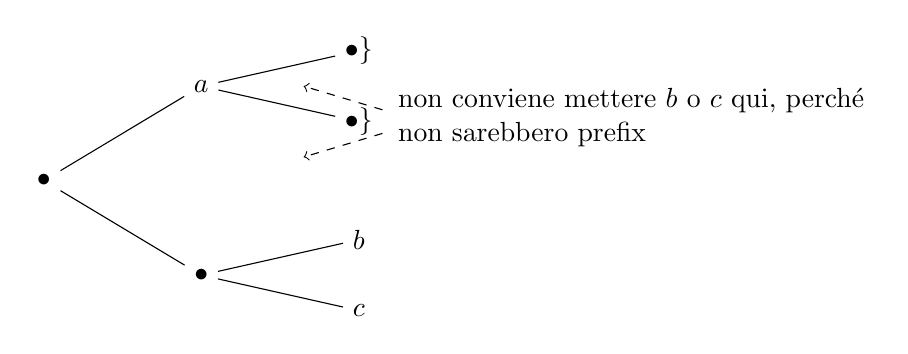
\begin{tikzpicture}[grow=right]
        \tikzstyle{level 2}=[sibling distance=.9cm]
        \node {$\bullet$}
        child {
            node {$\bullet$}
            child {
                node {$c$}
                edge from parent
            }
            child {
                node {$b$}
                edge from parent
            }    
            edge from parent
        }
        child {
            node {$a$}
            child {
                node {$\bullet\}$}
                edge from parent
            }
            child {
                node {$\bullet\}$}
                edge from parent
            }
            edge from parent
        };
    \node[text width=6cm,align=left] at (7.5,.8) {non conviene mettere $b$ o $c$ qui, perché non sarebbero prefix};
    \draw[->] (4.3,.9) node {} -- (3.3,1.2) [dashed] node {};
    \draw[->] (4.3,.6) node {} -- (3.3,.3) [dashed] node {};
    \end{tikzpicture}
\end{center}

\begin{theorem}[Teorema Diretto]
    $$
        \sum_{i=1}^k D^{-l_i} \leq 1
        \quad \Rightarrow \quad
        \exists \varphi \text{ prefisso con lunghezze } l_1,\dots,l_k
    $$
\end{theorem}
Prefisso è più forte di UD.\medskip 

I due risultati (teoremi) affermano che, anche se ci limitiamo all'utilizzo di codici prefisso, non perdiamo alcuna potenza nella compressione. È sufficiente l'utilizzo dei codici prefisso, comprimono a sufficienza.

\paragraph{Dimostrazione Teorema Inverso, caso prefisso + Teorema Diretto} Sia $\varphi$ un codice prefisso e $l_1\leq l_2\leq\dots\leq l_k=l$. Consideriamo l'albero $D$-ario (ogni nodo ha $D$ figli) che rappresenta $\varphi$, di altezza $l$.
\begin{center}
    \begin{tikzpicture}[grow=right]
        \tikzstyle{level 2}=[sibling distance=.5cm]
        \node {$\bullet$}
        child {
            node {$\bullet$}
            child {
                [dotted] node[right] {$\dots\bullet$}
                edge from parent
            }
            child {
                [dotted] node[right] {$\dots\bullet$}
                edge from parent
            }
            child {
                [dotted] node[right] {$\dots\bullet$}
                edge from parent
            }    
            edge from parent
        }
        child {
            node {$\bullet$}
            child {
                [dotted] node[right] {$\dots\bullet$}
                edge from parent
            }
            child {
                [dotted] node[right] {$\dots\bullet$}
                edge from parent
            }
            child {
                [dotted] node[right] {$\dots\bullet$}
                edge from parent
            }
            edge from parent
        }
        child {
            node {$\bullet$}
            child {
                [dotted] node[right] {$\dots\bullet$}
                edge from parent
            }
            child {
                [dotted] node[right] {$\dots\bullet$}
                edge from parent
            }
            child {
                [dotted] node[right] {$\dots\bullet$}
                edge from parent
            }
            edge from parent
        };
    \draw[<->] (4,-2.5) node {} -- (0,-2.5) node {};
    \node[below] at (2,-2.5) {$l$};
    \end{tikzpicture}
\end{center}

La codifica più lunga $a_k$ è in una delle foglie. Supponiamo che la codifica $a_i$ sia in uno dei nodi interni. Nessuno dei nodi interni (e in particolare nessuna delle foglie) del sottoalbero con $a_i$ come radice può essere utilizzato per un'altra codifica.
\begin{center}
    \begin{tikzpicture}[grow=right]
        \tikzstyle{level 1}=[level distance=2cm,sibling distance=2.4cm]
        \tikzstyle{level 2}=[level distance=2cm,sibling distance=.8cm]
        \node {$\bullet$}
        child {
            node {$\bullet$}
            child {
                [dotted] node[right] {$\qquad\dots\qquad\bullet$}
                edge from parent
            }
            child {
                [dotted] node[right] {$\qquad\dots\qquad\bullet$}
                edge from parent
            }
            child {
                [dotted] node[right] {$\qquad\dots\qquad\bullet$}
                edge from parent
            }    
            edge from parent
        }
        child {
            node {$\bullet$}
            child {
                [dotted] node[right] {$\qquad\dots\qquad\bullet$}
                edge from parent
            }
            child {
                [dotted] node[right] {$\qquad\dots\qquad a_k$}
                edge from parent
            }
            child {
                [dotted] node[right] {$\qquad\dots\qquad\bullet$}
                edge from parent
            }
            edge from parent
        }
        child {
            node {$\bullet$}
            child {
                [dotted] node[right] {$a_i$}
                edge from parent
            }
            child {
                [dotted] node[right] {$\qquad\dots\qquad\bullet$}
                edge from parent
            }
            child {
                [dotted] node[right] {$\qquad\dots\qquad\bullet$}
                edge from parent
            }
            edge from parent
        };
        \node[isosceles triangle,
            isosceles triangle apex angle=30,
            draw,
            rotate=180,
            fill=Gray!30,
            minimum size=1cm] (T)at (6.1,1.65){};
        \node at (5.8,1.65) {\tiny VIETATO};
    \end{tikzpicture}
\end{center}
In un tale albero, il numero di foglie è pari a $D^l$. 
\begin{center}
    \begin{tikzpicture}[grow=right]
        \tikzstyle{level 2}=[sibling distance=.5cm]
        \node {$\bullet$}
        child {
            node {$\bullet$}
            child {
                [dotted] node[right] {$\dots\bullet$}
                edge from parent
            }
            child {
                [dotted] node[right] {$\dots\bullet$}
                edge from parent
            }
            child {
                [dotted] node[right] {$\dots\bullet$}
                edge from parent
            }    
            edge from parent
        }
        child {
            node {$\bullet$}
            child {
                [dotted] node[right] {$\dots\bullet$}
                edge from parent
            }
            child {
                [dotted] node[right] {$\dots\bullet$}
                edge from parent
            }
            child {
                [dotted] node[right] {$\dots\bullet$}
                edge from parent
            }
            edge from parent
        }
        child {
            node {$\bullet$}
            child {
                [dotted] node[right] {$\dots\bullet$}
                edge from parent
            }
            child {
                [dotted] node[right] {$\dots\bullet$}
                edge from parent
            }
            child {
                [dotted] node[right] {$\dots\bullet$}
                edge from parent
            }
            edge from parent
        };
    \draw[<->] (4.5,-2.1) node {} -- (4.5,2.1) node {};
    \node[right] at (4.5,0) {$D^l$};
    \end{tikzpicture}
\end{center}
Il numero di foglie di un sottoalbero che parte da un nodo interno $a_i$ è $D^{l-l_i}$.
\begin{center}
\begin{tikzpicture}
    \node[isosceles triangle,
        isosceles triangle apex angle=40,
        draw,
        rotate=180,
        fill=Gray!30,
        minimum size=2.5cm] (T)at (0,0){};
    \draw[<->] (-2.55,-1.5) node {} -- (.85,-1.5) node {};
    \node[below] at (-0.85,-1.5) {$l-l_i$};
    \node at (-2.55,0) {$\bullet$};
    \node[left] at (-2.55,0) {$a_i$};
    \node[right] at (.85,1) {$\bullet$};
    \node[right] at (.85,0.1) {$\vdots$};
    \node[right] at (.85,-1) {$\bullet$};
    \draw[<->] (1.6,1.25) node {} -- (1.6,-1.25) node {};
    \node[right] at (1.6,0) {$D^{l-l_i}$};
\end{tikzpicture}
\end{center}
Quindi, riassumendo:
\begin{center}
    \begin{tikzpicture}[grow=right]
        \tikzstyle{level 1}=[level distance=2cm,sibling distance=2.4cm]
        \tikzstyle{level 2}=[level distance=2cm,sibling distance=.8cm]
        \node {$\bullet$}
        child {
            node {$\bullet$}
            child {
                [dotted] node[right] {$\qquad\dots\qquad\bullet$}
                edge from parent
            }
            child {
                [dotted] node[right] {$\qquad\dots\qquad\bullet$}
                edge from parent
            }
            child {
                [dotted] node[right] {$\qquad\dots\qquad\bullet$}
                edge from parent
            }    
            edge from parent
        }
        child {
            node {$\bullet$}
            child {
                [dotted] node[right] {$\qquad\dots\qquad\bullet$}
                edge from parent
            }
            child {
                [dotted] node[right] {$\qquad\dots\qquad a_k$}
                edge from parent
            }
            child {
                [dotted] node[right] {$\qquad\dots\qquad\bullet$}
                edge from parent
            }
            edge from parent
        }
        child {
            node {$\bullet$}
            child {
                [dotted] node[right] {$a_i$}
                edge from parent
            }
            child {
                [dotted] node[right] {$\qquad\dots\qquad\bullet$}
                edge from parent
            }
            child {
                [dotted] node[right] {$\qquad\dots\qquad\bullet$}
                edge from parent
            }
            edge from parent
        };
        \node[isosceles triangle,
            isosceles triangle apex angle=30,
            draw,
            rotate=180,
            fill=Gray!30,
            minimum size=1cm] (T)at (6.1,1.65){};
        \draw[<->] (-.1,-4) node {} -- (6.4,-4) node {};
        \node[below] at (3.15,-4) {$l$};
        \draw[<->] (6.8,1.15) node {} -- (6.8,2.15) node {};
        \node[right] at (6.8,1.65) {$D^{l-l_i}$};
        \draw[<->] (8.2,-3.3) node {} -- (8.2,3.3) node {};
        \node[right] at (8.2,0) {$D^l$};
    \end{tikzpicture}
\end{center}
Scriviamo che la differenza tra il numero totale di foglie $D^l$ e il numero di foglie dei sottoalberi (ovvero il numero di foglie vietate a causa dei sottoalberi creati da ogni $a_i$) è maggiore o uguale a 1:
\begin{align*}
    D^l - \sum_{i=1}^{k-1} D^{l-l_i} & \geq 1\\
    D^l\left(1-\sum_{i=1}^{k-1} D^{-l_i}\right) & \geq 1\\
    1 - \sum_{i=1}^{k-1} D^{-l_i} & \geq D^{-l_k}\\
    1 & \geq \sum_{i=1}^k D^{-l_i} %\qquad \square
\end{align*}
\hfill $\square$\medskip

Per il \textbf{Teorema Diretto}, si può leggere la dimostrazione ``al contrario''. In altre parole, vengono date le istruzioni per costruire l'albero, ovvero si disegna l'albero completo e si inizia ad etichettare. Più precisamente, si prende $a_1$, lo si mette a lunghezza $l_1$, e fino alle foglie si segna il resto dell'albero (il sottoalbero con radice $a_1$) come vietato. Si continua così per tutti gli $a_i$. \hfill $\square$

\paragraph{Dimostrazione Teorema Inverso, caso $\bm{\varphi}$ UD} Siano $l_1\leq\dots\leq l_k=l$ le lunghezze delle codifiche di $a_1,\dots,a_k$. Consideriamo $\mathcal{N}(n,h)$ numero di stringhe su $\mathcal{A}^n$ (ovvero di lunghezza $n$) che hanno una codifica $\varphi$ UD di lunghezza $h$. Sia $|\mathcal{B}^h|=D^h$ (numero di stringhe di lunghezza $h$ su $\mathcal{B}$). Poiché $\varphi$ è UD, $\mathcal{N}(n,h)\leq D^h$.
$$
    \sum_{i=1}^k D^{-l_i} = D^{-l_1} + D^{-l_2} + \dots + D^{-l_k} 
$$

Studiamo la crescita di tale oggetto alla potenza di $n$, quando $n$ va ad infinito. Questo perché, se la somma è $>1$, allora la potenza va ad infinito; se la somma è $<1$, allora la potenza va a 0 (è limitata); se la somma è $=1$, allora la potenza va a 1.
$$
    \forall n \qquad \left(D^{-l_1} + D^{-l_2} + \dots + D^{-l_k}\right)^n \qquad (\text{chiamiamola }\alpha^n)
$$

Se si svolge l'elevamento a potenza di tale polinomio, si otterrà una serie di addendi del seguente tipo:
$$
    D^{-l_1\cdot n} +
    \dots +
    D^{(-l_1)+(-l_2)+(-l_1)+\dots} +
    \dots +
    D^{-l_k\cdot n}
$$
dove $-l_1\cdot n$ è la lunghezza della codifica della stringa $a_1a_1\dots a_1$, con $n$ ripetizioni di $a_1$, ovvero $|\varphi(a_1\dots a_1)|=l_1\cdot n$. Allo stesso modo, $-l_k\cdot n$ è la lunghezza della codifica della stringa $a_ka_k\dots a_k$, con $n$ ripetizioni di $a_k$. Un generico esponente all'interno, ad esempio $-(l_1+l_2+l_1+\dots)$ è una somma di lunghezze di codifiche, e ammonta alla lunghezza di una generica stringa. Ad esempio, $-(10)$, se chiamo $10=h$.

Si ha che $D^{-h}$ si verifica nella somma esattamente $\mathcal{N}(n,h)$ volte (alcune delle quali saranno 0). Quindi, la somma $D^{-l_1\cdot n}+\dots+D^{-l_k\cdot n}$ si può riscrivere come 
\begin{align*}
    \mathcal{N}(n,0)D^{-0} + \mathcal{N}(n,1)D^{-1} + \dots + \underbrace{\mathcal{N}(n,n\cdot l)}_{\geq 1}D^{-n\cdot l} & \quad\leq\quad
    D^0D^{-0} + D^1D^{-1} + \dots + D^{n\cdot l}D^{-n\cdot l}\\
    1+1+\dots+1 & \quad\leq\quad n\cdot l + 1\\
    \forall n \qquad \alpha^n &\quad\leq\quad \underbrace{l}_{costante}\cdot~ n
\end{align*}
Da cui si ricava
$$
    \alpha \leq 1
$$
Quindi
$$
    \sum_{i=1}^k D^{-l_i} \leq 1
$$
\hfill $\square$



\subsection{Compressione Massima}
La sorgente che genera il messaggio del codice è stazionaria e senza memoria (Fig.~\vref{fig:shannon-paper}).
\begin{figure}[htb]
    \centering
    \includegraphics[width=.7\textwidth]{figures/shannon-paper.png}
    \caption{Diagramma schematico di un sistema di comunicazione, da C.~E.~Shannon, \textit{A Mathematical Theory of Communication}, Bell System Technical Journal, 1948.}
    \label{fig:shannon-paper}
\end{figure}
Poiché il messaggio codificato deve passare attraverso un canale, il quale ha una sua capacità e una sua velocità, lo si vuole comprimere il più possibile.

Ricordiamo che 
$$
    P=\{p_1,\dots,p_k\} \qquad \mathcal{A}=\{a_1,\dots,a_k\} \qquad l_i=|\varphi(a_i)| \qquad EL(\varphi) = \sum_{i=1}^k p_il_i
$$

\begin{theorem}[$\bm{1^\circ}$ Shannon]
    $$
        \varphi \text{ è UD} \quad \Rightarrow \quad EL(\varphi) \geq \mathcal{H}_D(P)
    $$

    con 
    $$
        \mathcal{H}_D(P) = \sum_{i=1}^k p_i\cdot\log_D\frac{1}{p_i}
    $$
\end{theorem}

\paragraph{Dimostrazione} 
\begin{align*}
    EL(\varphi)-\mathcal{H}_D(P) &= \sum_{i=1}^k p_i\underbrace{l_i}_{\log_DD^{l_i}} + \sum_{i=1}^k p_i\cdot\log_Dp_i\\
    &= \sum_{i=1}^k p_i\cdot\log_D(D^{l_i}\cdot p_i)\\
\end{align*}
Prima di proseguire, ricordiamo la seguente proprietà dei logaritmi su $\mathbb{N}$:
$$
    \log_ex\leq x-1; \qquad -\log_ex\geq -(x-1) 
$$
e anche la proprietà dei logaritmi:
$$
    \log_bx = \frac{\log_cx}{\log_cb}
$$
Continuiamo la dimostrazione:
\begin{align*}
    EL(\varphi)-\mathcal{H}_D(P) &= \sum_{i=1}^k p_i\cdot\log_D(D^{l_i}\cdot p_i)\\
    &= \frac{1}{log_eD} \sum_{i=1}^k p_i\cdot\log_e(D^{l_i}\cdot p_i)\\
    &= -\frac{1}{\log_eD} \sum_{i=1}^k p_i\cdot\log_e\left(\frac{1}{D^{l_i}\cdot p_i}\right)\\
    &\geq -\frac{1}{\log_eD} \sum_{i=1}^k p_i\cdot\left(\frac{1}{D^{l_i}\cdot p_i}-1\right)\\
    &= -\frac{1}{\log_eD} \underbrace{\left(\sum_{i=1}^k\frac{1}{D^{l_i}}-\underbrace{1}_{\sum p_i}\right)}_{\leq 0}\\
    &\geq 0
\end{align*}
\hfill $\square$ 


% LEZIONE 5
\subsection{Shannon Code}
Dal Teorema $1^\circ$ Shannon abbiamo:
$$
EL(\varphi) = \sum_{i=1}^k p_il_i ~ \geq ~ \mathcal{H}_D(P) = \sum_{i=1}^k p_i\log_D\frac{1}{p_i}
$$
La differenza sta in $l_i$ e $\log_D\frac{1}{p_i}$, quindi vogliamo provare ad eguagliarli:
$$
    l_i = \log_D\frac{1}{p_i}
$$
Ma $\log_D\frac{1}{p_i}$ non è necessariamente intero. Decidiamo quindi di considerare il suo primo intero più grande:
$$
l_i = \left\lceil\log_D\frac{1}{p_i}\right\rceil = \left\lceil-\log_Dp_i\right\rceil
$$
È sempre possibile definire un codice UD con tali lunghezze? Possiamo utilizzare Kraft-McMillan. Vogliamo controllare se
$$
    \sum_{i=1}^k D^{-\lceil-\log_Dp_i\rceil}
    \stackrel{?}{\leq}
    1
$$
Sappiamo che 
$$
    \lceil-\log_Dp_i\rceil = -log_Dp_i+\beta_i \qquad\qquad 0\leq\beta_i<1
$$
Quindi possiamo scrivere
\begin{align*}
    \sum_{i=1}^k D^{-(-log_Dp_i+\beta_i)} &= \sum_{i=1}^k D^{log_Dp_i}\cdot D^{\beta_i}\\
    &= \sum_{i=1}^k p_i\cdot D^{-\beta_i}\\
    &= \sum_{i=1}^k p_i\cdot \frac{1}{D^{\beta_i}}
\end{align*}
Ricordiamo che $0\leq\beta_i<1$ e $D>1$, di conseguenza $\frac{1}{D^{\beta_i}}\leq 1$. Quindi
\begin{align*}
    \sum_{i=1}^k p_i\cdot \frac{1}{D^{\beta_i}} &\leq 1\\
    \sum_{i=1}^k D^{-\lceil-\log_Dp_i\rceil} &\leq 1
\end{align*}
Esiste quindi un prefix code con lunghezze $l_i=\lceil-\log_Dpi\rceil$ definibile utilizzando una strategia greedy sull'albero $D$-ario.
\begin{center}
    \begin{tikzpicture}[grow=right]
        \tikzstyle{level 1}=[level distance=2cm,sibling distance=2cm]
        \tikzstyle{level 2}=[level distance=2cm,sibling distance=1.2cm]
        \node {$\bullet$}
        child {
            [dotted] node { }
            edge from parent
        }
        child {
            node {$\bullet$}
            edge from parent
        }
        child {
            node {$\bullet$}
            child {
                [dotted] node[right] { }
                edge from parent
            }
            child {
                [dotted] node[right] { }
                edge from parent
            }
            child {
                [dotted] node[right] {$\varphi(a_1)$}
                edge from parent
            }
            edge from parent
        };

        \draw [decorate,
            decoration = {brace,amplitude=10pt}] (-0.2,0.3) -- (3.8,3.5);
        \node[rotate=40] at (1.3,2.4) {$\lceil-\log_Dp_1\rceil$};
    \end{tikzpicture}
\end{center}

\paragraph{Esempio} Siano $\mathcal{A}=\{a,b\}$, $\mathcal{B}=\{0,1\}$, $P=\{1-\frac{1}{32},\frac{1}{32}\}$. Abbiamo che
$$
    l_2 = -\log_232 = 5 \qquad\qquad l_1 = \left\lceil -\log_2\left(1-\frac{1}{32}\right)\right\rceil = 1
$$
Ciò significa che lo shannon code codifica l'alfabeto come
$$
    \varphi(a) = 0 \qquad\qquad \varphi(b) = 10000
$$
\begin{center}
    \begin{tikzpicture}[grow=right]
        \node {$\bullet$}
        child {
            node {$\bullet$}
            child {
                    node {$\bullet$}
                    child {
                        node {$\bullet$}
                        child {
                            node {$\bullet$}
                            child {
                                node {$b$}
                                edge from parent
                                node[below] {$0$}
                            }
                            edge from parent
                            node[below] {$0$}
                        }
                        edge from parent
                        node[below] {$0$}
                    }
                    edge from parent
                    node[below] {$0$}
                }     
            edge from parent 
            node[below] {$1$}
        }
        child {
            node {$a$}
            edge from parent         
            node[above] {$0$}
        };
    \end{tikzpicture}
\end{center}



\textcolor{Red}{TODO: finire lezione 5}

\textcolor{Red}{TODO: osservazione su $\varphi_{SF}$ in appunti lez 6}


% LEZIONE 6
\begin{definition}[Efficienza (Efficiency of code)]
    $$
        Eff(\varphi) = \frac{\mathcal{H}_D(P)}{EL(\varphi)}
    $$
\end{definition}
\emph{Eff} è sempre $\leq 1$, e ci dice quanto siamo vicini all'entropia, che non è sempre raggiungibile.\medskip

Ci chiediamo perché Huffmann (merge delle foglie) è ottimale, mentre Shannon-Fano (splitting dalla radice) non lo è?


\section{Codici Stream}
Capitolo 6 del libro di MacKay. In questo capitolo discuteremo uno schema di compressione dei dati. La codifica Lempel-Ziv è un metodo ``universale'', progettato secondo la filosofia per cui vorremmo un unico algoritmo di compressione che faccia un lavoro ragionevole per qualsiasi fonte. In effetti, per molte fonti della vita reale, le proprietà universali di questo algoritmo valgono solo nel limite di quantità di dati eccessivamente grandi, ma, comunque, la compressione Lempel-Ziv è ampiamente utilizzata e spesso efficace.


\subsection{Un po' di Storia}
\textcolor{Red}{TODO: scrivere la storia}


\subsection{Lempel-Ziv}
Immaginiamo un messaggio come uno stream (vettore) di caratteri su $\mathcal{A}^*$.

\begin{center}
    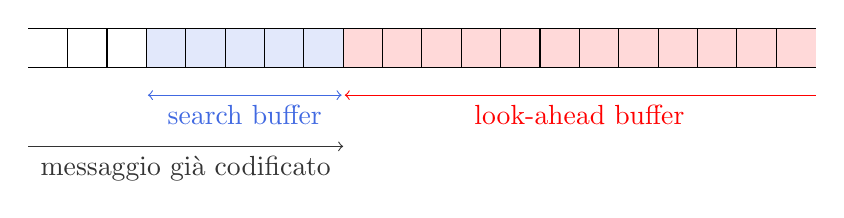
\begin{tikzpicture}%[scale=0.5]
        % buffers
        \draw[fill=RoyalBlue!15,draw=none] (1.5,0) rectangle (4,0.5);
        \draw[fill=Red!15,draw=none] (4,0) rectangle (10,0.5);

        % Draw the horizontal strip
        \draw (0,0) -- (10,0);
        \draw (0,.5) -- (10,.5);
      
        % Draw the squares
        \foreach \x in {0.5,1,...,9.5} {
          \draw (\x,0) -- (\x,.5);
        }

        \draw[<->,color=RoyalBlue] (1.52,-.35) -- (3.98,-.35);
        \node[below,color=RoyalBlue] at (2.75,-.35) {search buffer};
        \draw[<-,color=Red] (4.02,-.35) -- (10,-.35);
        \node[below,color=Red] at (7,-.35) {look-ahead buffer};
        \draw[->,color=Black!80] (0,-1) -- (4,-1);
        \node[below,color=Black!80] at (2,-1) {messaggio già codificato};
    \end{tikzpicture}
\end{center}
Cerchiamo il prefisso più lungo del look-ahead buffer che sia presente nel search buffer. Se lo troviamo, lo sostituiamo con un puntatore alla sua posizione nel search buffer e la sua lunghezza. Se non lo troviamo, scriviamo il carattere e passiamo al carattere successivo.

Ad ogni iterazione, l'algoritmo produce triple della forma $(o,l,s)$, dove
\begin{itemize}
    \item $o$ è l'offset, ovvero la distanza tra $i$ (primo carattere del look-ahead buffer) e $j$ (primo carattere del prefisso nel search buffer)
    \item $l$ è la lunghezza del prefisso
    \item $s$ è il primo carattere mismatching
\end{itemize}
\begin{center}
    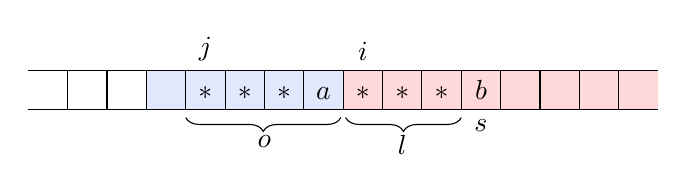
\begin{tikzpicture}%[scale=0.5]
        % buffers
        \draw[fill=RoyalBlue!15,draw=none] (1.5,0) rectangle (4,0.5);
        \draw[fill=Red!15,draw=none] (4,0) rectangle (8,0.5);

        % Draw the horizontal strip
        \draw (0,0) -- (8,0);
        \draw (0,.5) -- (8,.5);
      
        %  Draw the squares
        \foreach \x in {0.5,1,...,7.5} {
          \draw (\x,0) -- (\x,.5);
        }

        % Label the squares
        \foreach \x in {2.25,2.75,3.25,4.25,4.75,5.25} {
          \node[above] at (\x,0) {$*$};
        }
        \node[above] at (3.75,0) {$a$};
        \node[above] at (5.75,0) {$b$};

        \draw [decorate,
            decoration = {brace,mirror,amplitude=5pt}] (4.03,-0.1) -- (5.5,-0.1);
        \node[below] at (4.75,-0.2) {$l$};
        \draw [decorate,
            decoration = {brace,mirror,amplitude=5pt}] (2,-0.1) -- (3.97,-0.1);
        \node[below] at (3,-0.2) {$o$};
        \node[above] at (2.25,0.5) {$j$};
        \node[above] at (4.25,0.5) {$i$};
        \node[below] at (5.75,0) {$s$};
    \end{tikzpicture}
\end{center}

\subsubsection{LZ77}
Abbiamo un search buffer di lunghezza 5, e la stringa $babbababbabbabba$. All'inizio, il search buffer è vuoto, e possiamo quindi immaginarlo con caratteri al di fuori dell'alfabeto.
\begin{center}
    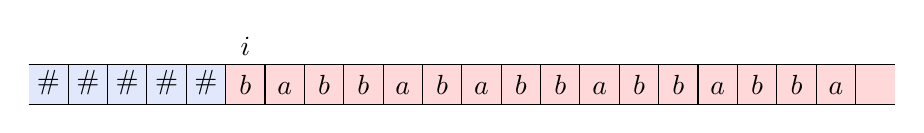
\begin{tikzpicture}%[scale=0.5]
        % buffers
        \draw[fill=RoyalBlue!15,draw=none] (0,0) rectangle (2.5,0.5);
        \draw[fill=Red!15,draw=none] (2.5,0) rectangle (11,0.5);

        % Draw the horizontal strip
        \draw (0,0) -- (11,0);
        \draw (0,.5) -- (11,.5);
      
        %  Draw the squares
        \foreach \x in {0.5,1,...,10.5} {
          \draw (\x,0) -- (\x,.5);
        }

        % Label the squares
        \foreach \x in {0.25,0.75,...,2.25} {
          \node[above] at (\x,0) {$\#$};
        }

        \foreach \x/\y in {2.75/$b$,3.25/$a$,3.75/$b$,4.25/$b$,4.75/$a$,5.25/$b$,5.75/$a$,6.25/$b$,6.75/$b$,7.25/$a$,7.75/$b$,8.25/$b$,8.75/$a$,9.25/$b$,9.75/$b$,10.25/$a$} {
          \node[above] at (\x,0) {\y};
        }

        % \node[above] at (2.25,0.5) {$j$};
        \node[above] at (2.75,0.5) {$i$};
    \end{tikzpicture}
\end{center}
La prima tripla $(o,l,s)$ della codifica è quindi $(0,0,b)$. Proseguiamo spostando il search buffer di un carattere a destra:
\begin{center}
    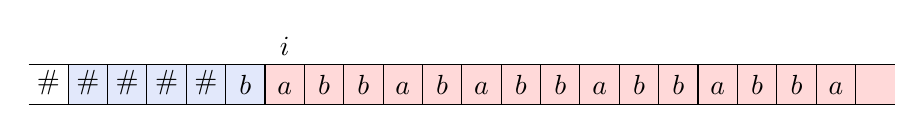
\begin{tikzpicture}%[scale=0.5]
        % buffers
        \draw[fill=RoyalBlue!15,draw=none] (0.5,0) rectangle (3,0.5);
        \draw[fill=Red!15,draw=none] (3,0) rectangle (11,0.5);

        % Draw the horizontal strip
        \draw (0,0) -- (11,0);
        \draw (0,.5) -- (11,.5);
      
        %  Draw the squares
        \foreach \x in {0.5,1,...,10.5} {
          \draw (\x,0) -- (\x,.5);
        }

        % Label the squares
        \foreach \x in {0.25,0.75,...,2.25} {
          \node[above] at (\x,0) {$\#$};
        }

        \foreach \x/\y in {2.75/$b$,3.25/$a$,3.75/$b$,4.25/$b$,4.75/$a$,5.25/$b$,5.75/$a$,6.25/$b$,6.75/$b$,7.25/$a$,7.75/$b$,8.25/$b$,8.75/$a$,9.25/$b$,9.75/$b$,10.25/$a$} {
          \node[above] at (\x,0) {\y};
        }

        % \node[above] at (2.25,0.5) {$j$};
        \node[above] at (3.25,0.5) {$i$};
    \end{tikzpicture}
\end{center}
Il prefisso del look-ahead buffer inizia per $a$, e quindi non è presente nel search buffer. La seconda tripla è $(0,0,a)$, e il search buffer viene spostato di un carattere a destra:
\begin{center}
    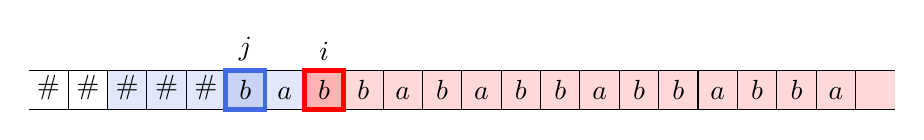
\begin{tikzpicture}%[scale=0.5]
        % buffers
        \draw[fill=RoyalBlue!15,draw=none] (1,0) rectangle (3.5,0.5);
        \draw[fill=Red!15,draw=none] (3.5,0) rectangle (11,0.5);

        % Draw the horizontal strip
        \draw (0,0) -- (11,0);
        \draw (0,.5) -- (11,.5);
      
        %  Draw the squares
        \foreach \x in {0.5,1,...,10.5} {
          \draw (\x,0) -- (\x,.5);
        }

        \draw[color=RoyalBlue,fill=RoyalBlue!30,ultra thick] (2.5,0) rectangle (3,0.5);
        \draw[color=Red,fill=Red!30,ultra thick] (3.5,0) rectangle (4,0.5);

        % Label the squares
        \foreach \x in {0.25,0.75,...,2.25} {
          \node[above] at (\x,0) {$\#$};
        }

        \foreach \x/\y in {2.75/$b$,3.25/$\cancel{a}$,3.75/$b$,4.25/$\cancel{b}$,4.75/$a$,5.25/$b$,5.75/$a$,6.25/$b$,6.75/$b$,7.25/$a$,7.75/$b$,8.25/$b$,8.75/$a$,9.25/$b$,9.75/$b$,10.25/$a$} {
          \node[above] at (\x,0) {\y};
        }

        \node[above] at (2.75,0.5) {$j$};
        \node[above] at (3.75,0.5) {$i$};
    \end{tikzpicture}
\end{center}
Confrontiamo nuovamente il prefisso del look-ahead buffer con il search buffer. Il prefisso inizia per $b$, che è presente anche nel search buffer. Continua con $b$, ma nel search buffer la $b$ è seguita da una $a$. Il prefisso è quindi $b$, di lunghezza 1, la distanza tra $j$ e $i$ è 2, e il primo carattere mismatching è $b$. La terza tripla è quindi $(2,1,b)$, e il search buffer viene spostato di due caratteri a destra:
\begin{center}
    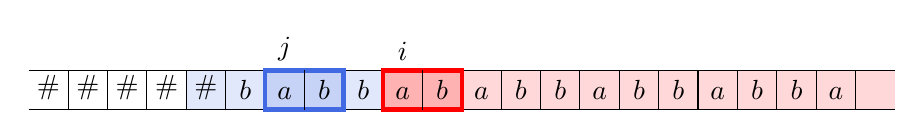
\begin{tikzpicture}%[scale=0.5]
        % buffers
        \draw[fill=RoyalBlue!15,draw=none] (2,0) rectangle (4.5,0.5);
        \draw[fill=Red!15,draw=none] (4.5,0) rectangle (11,0.5);

        % Draw the horizontal strip
        \draw (0,0) -- (11,0);
        \draw (0,.5) -- (11,.5);

        \draw[color=RoyalBlue,fill=RoyalBlue!30,ultra thick] (3,0) rectangle (4,0.5);
        \draw[color=Red,fill=Red!30,ultra thick] (4.5,0) rectangle (5.5,0.5);
      
        %  Draw the squares
        \foreach \x in {0.5,1,...,10.5} {
          \draw (\x,0) -- (\x,.5);
        }

        \draw[color=RoyalBlue,ultra thick] (3,0) -- (3,.5);
        \draw[color=RoyalBlue,ultra thick] (4,0) -- (4,.5);
        \draw[color=Red,ultra thick] (4.5,0) -- (4.5,.5);
        \draw[color=Red,ultra thick] (5.5,0) -- (5.5,.5);

        % Label the squares
        \foreach \x in {0.25,0.75,...,2.25} {
          \node[above] at (\x,0) {$\#$};
        }

        \foreach \x/\y in {2.75/$b$,3.25/$a$,3.75/$b$,4.25/$\cancel{b}$,4.75/$a$,5.25/$b$,5.75/$\cancel{a}$,6.25/$b$,6.75/$b$,7.25/$a$,7.75/$b$,8.25/$b$,8.75/$a$,9.25/$b$,9.75/$b$,10.25/$a$} {
          \node[above] at (\x,0) {\y};
        }

        \node[above] at (3.25,0.5) {$j$};
        \node[above] at (4.75,0.5) {$i$};
    \end{tikzpicture}
\end{center}
Anche in questo caso cominciamo a guardare i caratteri del look-ahead buffer, e cerchiamo il più lungo prefisso presente anche nel search buffer. Il prefisso è $ab$ (lunghezza 2), la distanza tra $j$ e $i$ è 3, e il primo carattere mismatching è una $a$. La tripla è quindi $(3,2,a)$, e proseguiamo spostando il search buffer di tre caratteri a destra. Gli ultimi due passaggi sono i seguenti:
\begin{center}
    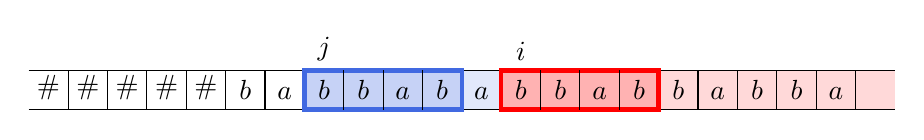
\begin{tikzpicture}%[scale=0.5]
        % buffers
        \draw[fill=RoyalBlue!15,draw=none] (3.5,0) rectangle (6,0.5);
        \draw[fill=Red!15,draw=none] (6,0) rectangle (11,0.5);

        % Draw the horizontal strip
        \draw (0,0) -- (11,0);
        \draw (0,.5) -- (11,.5);

        \draw[color=RoyalBlue,fill=RoyalBlue!30,ultra thick] (3.5,0) rectangle (5.5,0.5);
        \draw[color=Red,fill=Red!30,ultra thick] (6,0) rectangle (8,0.5);
      
        %  Draw the squares
        \foreach \x in {0.5,1,...,10.5} {
          \draw (\x,0) -- (\x,.5);
        }

        \draw[color=RoyalBlue,ultra thick] (3.5,0) -- (3.5,.5);
        \draw[color=RoyalBlue,ultra thick] (5.5,0) -- (5.5,.5);
        \draw[color=Red,ultra thick] (6,0) -- (6,.5);
        \draw[color=Red,ultra thick] (8,0) -- (8,.5);

        % Label the squares
        \foreach \x in {0.25,0.75,...,2.25} {
          \node[above] at (\x,0) {$\#$};
        }

        \foreach \x/\y in {2.75/$b$,3.25/$a$,3.75/$b$,4.25/$b$,4.75/$a$,5.25/$b$,5.75/$\cancel{a}$,6.25/$b$,6.75/$b$,7.25/$a$,7.75/$b$,8.25/$\cancel{b}$,8.75/$a$,9.25/$b$,9.75/$b$,10.25/$a$} {
          \node[above] at (\x,0) {\y};
        }

        \node[above] at (3.75,0.5) {$j$};
        \node[above] at (6.25,0.5) {$i$};
    \end{tikzpicture}
\end{center}
\begin{center}
    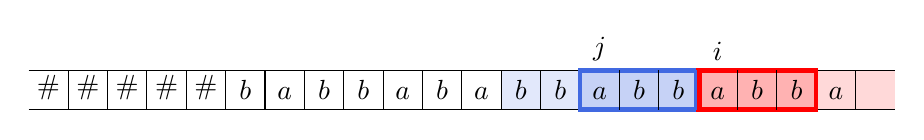
\begin{tikzpicture}%[scale=0.5]
        % buffers
        \draw[fill=RoyalBlue!15,draw=none] (6,0) rectangle (8.5,0.5);
        \draw[fill=Red!15,draw=none] (8.5,0) rectangle (11,0.5);

        % Draw the horizontal strip
        \draw (0,0) -- (11,0);
        \draw (0,.5) -- (11,.5);

        \draw[color=RoyalBlue,fill=RoyalBlue!30,ultra thick] (7,0) rectangle (8.5,0.5);
        \draw[color=Red,fill=Red!30,ultra thick] (8.5,0) rectangle (10,0.5);
      
        %  Draw the squares
        \foreach \x in {0.5,1,...,10.5} {
          \draw (\x,0) -- (\x,.5);
        }

        \draw[color=RoyalBlue,ultra thick] (7,0) -- (7,.5);
        \draw[color=RoyalBlue,ultra thick] (8.48,0) -- (8.48,.5);
        \draw[color=Red,ultra thick] (8.52,0) -- (8.52,.5);
        \draw[color=Red,ultra thick] (10,0) -- (10,.5);

        % Label the squares
        \foreach \x in {0.25,0.75,...,2.25} {
          \node[above] at (\x,0) {$\#$};
        }

        \foreach \x/\y in {2.75/$b$,3.25/$a$,3.75/$b$,4.25/$b$,4.75/$a$,5.25/$b$,5.75/$a$,6.25/$b$,6.75/$b$,7.25/$a$,7.75/$b$,8.25/$b$,8.75/$a$,9.25/$b$,9.75/$b$,10.25/$\cancel{a}$} {
          \node[above] at (\x,0) {\y};
        }

        \node[above] at (7.25,0.5) {$j$};
        \node[above] at (8.75,0.5) {$i$};
    \end{tikzpicture}
\end{center}
Corrispondenti alle triple $(5,4,b)$ e $(3,3,a)$ rispettivamente.

La codifica del messaggio $babbababbabbabba$ con l'algoritmo LZ77 è quindi rappresentata dalla sequenza di triple $(0,0,b)(0,0,a)(2,1,b)(3,2,a)(5,4,b)(3,3,a)$.\bigskip

L'esempio appena mostrato utilizza un messaggio piuttosto corto, e quindi non è possibile apprezzare la compressione. Per messaggi più lunghi, la dimensione delle triple è molto più piccola della dimensione del messaggio originale.

In quale caso LZ77 comprime molto? Immaginiamo di avere il messaggio $aaaaaaaaaaaaaaab$. Il primo mismatch si trova solo all'ultimo carattere, tutta la parte di ripetizione di $a$ è il prefisso più lungo. Nel caso migliore, si può ottenere una compressione esponenziale.

Per questo tipo di codifica, il decodificatore deve essere a conoscenza dell'alfabeto e della lunghezza del search buffer. Più precisamente, deve avere un buffer di lunghezza almeno pari alla lunghezza del buffer del codificatore.

% LEZIONE 7
\paragraph{Note} La sorgente che genera le lettere del messaggio è stazionaria e senza memoria. Le probabilità non cambiano nel tempo. 

LZ esegue i cambiamenti sulle probabilità durante la codifica, mentre S e SF no. Questi ultimi due dovrebbero costruire un altro albero se le probabilità cambiano.




\chapter{Codifica di Canale Rumoroso}

\section{Variabili Aleatorie Dipendenti}
Capitolo 8 del libro di MacKay. Negli precedenti capitoli sulla compressione dei dati ci siamo concentrati sui vettori aleatori $x$ provenienti da una distribuzione di probabilità estremamente semplice, ovvero la distribuzione separabile in cui ciascuna componente $x_n$ è indipendente dalle altre.

In questo capitolo considereremo insiemi congiunti in cui le variabili aleatorie sono dipendenti. Questo materiale ha due motivazioni. Innanzitutto, i dati del mondo reale hanno correlazioni interessanti, quindi per eseguire una buona compressione dei dati, dobbiamo sapere come lavorare con modelli che includono dipendenze. In secondo luogo, un canale rumoroso con input $x$ e output $y$ definisce un insieme congiunto in cui $x$ e $y$ sono dipendenti (se fossero indipendenti, sarebbe impossibile comunicare sul canale) quindi la comunicazione sui canali rumorosi è descritto in termini di entropia degli insiemi congiunti.

\subsection{Divergenza e Disuguagianza di Gibbs}
La divergenza di Kullback-Leibler è una misura della differenza tra due distribuzioni di probabilità. Siano $P$ e $Q$ due distribuzioni di probabilità su $X$. La divergenza di Kullback-Leibler tra $P$ e $Q$ è definita come
\begin{align*}
    D(P||Q) &= \sum_{x\in X} P(x)\log\left(\frac{P(x)}{Q(x)}\right)\\
    &= \sum_{x\in X} P(x) \left( \log\left(\frac{1}{Q(x)}\right) - \log\left(\frac{1}{P(x)}\right) \right)
\end{align*}
Notiamo che $\sum_{x\in X} P(x)\log\left(\frac{P(x)}{Q(x)}\right)$ è il vaore atteso di $\log\left(\frac{P(x)}{Q(x)}\right)$ rispetto a $P$. Inoltre, $\log\left(\frac{P(x)}{Q(x)}\right)$ può essere espresso come $\log\left(\frac{1}{Q(x)}\right) - \log\left(\frac{1}{P(x)}\right)$, con $-P(x)\log\left(\frac{1}{P(x)}\right)$ entropia della distribuzione $P$.

Il significato della divergenza, in questo contesto, è ``quanti bit in più devo usare per codificare una sorgente utilizzando $Q$ al posto di $P$'', con $P$ distribuzione reale dei dati.

\paragraph{Esempio} Se si hanno dei caratteri con probabilità 0, si utilizzerà per essi una codifica molto lunga, così da conservare codifiche brevi per altri caratteri con probabilità maggiori.
\begin{align*}
    \mathcal{A} &= \{a,b,c,d,e\}\\
    P &= \{\dots,\dots,\dots,0,0\}\\
    Q &= \{0.2,0.2,0.2,0.2,0.2\}
\end{align*}
Non conosciamo la distribuzione reale dei dati $P$, ma abbiamo dedotto $Q$.

\paragraph{Proprietà} La divergenza non è simmetrica.
$$
    D(P||Q) \neq D(Q||P)
$$
La divergenza è sempre non negativa, e vale 0 se e solo se $P=Q$.
$$
    D(P||Q) \geq 0 \qquad\qquad D(P||Q) = 0 \Leftrightarrow P=Q
$$
Quest'ultima proprietà è una conseguenza della \textbf{disuguaglianza di Gibbs}.


\subsection{Entropia e Mutual Information}
Siano $X,Y$ variabili aleatorie. Come abbiamo già visto, l'entropia congiunta è 
$$
    \mathcal{H}(X,Y) = \sum_{\substack{x\in X\\y\in Y}} p(x,y)\log \left(\frac{1}{p(x,y)}\right)
$$
L'entropia è additiva sse $X$ e $Y$ sono indipendenti
$$
    \mathcal{H}(X,Y) = \mathcal{H}(X) + \mathcal{H}(Y)
    \quad \Leftrightarrow \quad
    p(x,y) = p(x)p(y)
$$
L'entropia condizionale di $X$ dato $Y=y$, ovvero se si conosce il valore di una delle due variabili, è l'entropia della distribuzione di probabilità $P(x|y)$
$$
    \mathcal{H}(X|Y=y) = \sum_{x\in X} p(x|y)\log \left(\frac{1}{p(x|y)}\right)
$$
L'entropia condizionale di $X$ dato $Y$ è la media, su tutti i valori di $Y$, dell'entropia condizionale di $X$ dato $Y=y$.
L'incertezza del valore di $X$ se si conosce il valore di $Y$ è quindi
\begin{align*}
    \mathcal{H}(X|Y) &= \sum_{y\in Y} p(y)\mathcal{H}(X|Y=y)\\
    &= \sum_{\substack{x\in X\\y\in Y}} p(x,y)\log \left(\frac{1}{p(x|y)}\right)
\end{align*}


\paragraph{$\bm{X}$ e $\bm{Y}$ indipendenti} Se $X$ e $Y$ sono indipendenti, allora
\begin{align*}
    p(x,y) &= p(x)p(y)\\
    p(x|y) = p(x) \quad &\Rightarrow \quad \mathcal{H}(X,Y) = \mathcal{H}(X)
\end{align*}
(Dimostrare che se $X$ e $Y$ sono indipendenti, allora $\mathcal{H}(X,Y) = \mathcal{H}(X)$)

\paragraph{$\bm{X}$ e $\bm{Y}$ dipendenti} Conosciuta anche come \emph{chain rule} per l'entropia. L'entropia congiunta, $\mathcal{H}(X,Y)$, l'entropia condizionale, $\mathcal{H}(X|Y)$ o $\mathcal{H}(Y|X)$, e l'entropia marginale, $\mathcal{H}(X)$ o $\mathcal{H}(Y)$, sono legate dalla seguente relazione
\begin{align*}
    \mathcal{H}(X,Y) &= \mathcal{H}(X) + \mathcal{H}(Y|X)\\
    &= \mathcal{H}(Y) + \mathcal{H}(X|Y)
\end{align*}
Abbiamo un analogo al caso delle probabilità, solo con l'addizione al posto della moltiplicazione, in quanto passiamo alla funzione logaritmo.


\subsubsection{Mutual Information}
La \textbf{mutual information} è una misura della dipendenza tra due variabili aleatorie. È definita come
\begin{align*}
    I(X,Y) &= \mathcal{H}(X) - \mathcal{H}(X|Y)\\
    &= \mathcal{H}(Y) - \mathcal{H}(Y|X)
\end{align*}
Misura la riduzione media dell'incertezza su $X$ se si conosce il valore di $Y$, o viceversa. 
Vale che $I(X,Y)\geq0$, e in particolare $I(X,Y)=0$ se $X$ e $Y$ sono indipendenti. 
Inoltre, $I(X,Y)$ è massimo quando l'incertezza su $X$ se si conosce $Y$ (o viceversa) è nulla:
$$
    X=Y \quad \Rightarrow \quad \mathcal{H}(X|Y)=0 \quad \Rightarrow \quad I(X,Y) = \mathcal{H}(X)
$$

\paragraph{Rappresentazione visuale} $I(X,Y) = \mathcal{H}(X) + \mathcal{H}(Y) - \mathcal{H}(X,Y)$
\begin{center}
    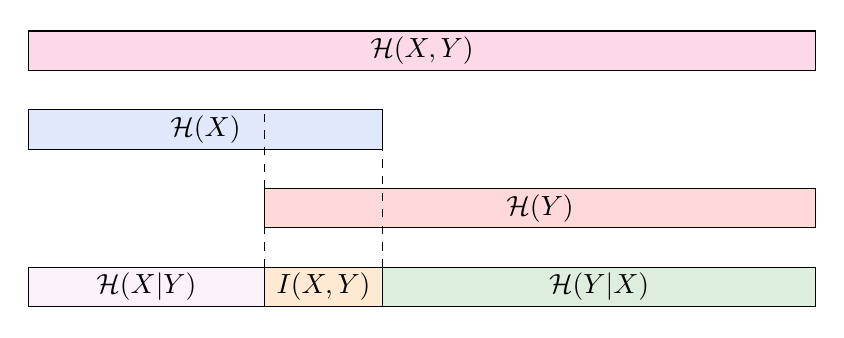
\begin{tikzpicture}%[scale=0.5]
        % H(X,Y)
        \draw[fill=RubineRed!15] (0,0) rectangle (10,0.5);
        \node at (5,0.25) {$\mathcal{H}(X,Y)$};

        % H(X)
        \draw[fill=RoyalBlue!15] (0,-1) rectangle (4.5,-0.5);
        \node at (2.25,-0.75) {$\mathcal{H}(X)$};

        % H(Y)
        \draw[fill=Red!15] (3,-2) rectangle (10,-1.5);
        \node at (6.5,-1.75) {$\mathcal{H}(Y)$};

        % H(X|Y)
        \draw[fill=Plum!15] (0,-3) rectangle (3,-2.5);
        \node at (1.5,-2.75) {$\mathcal{H}(X|Y)$};

        % I(X,Y)
        \draw[fill=BurntOrange!15] (3,-3) rectangle (4.5,-2.5);
        \node at (3.75,-2.75) {$I(X,Y)$};

        % H(Y|X)
        \draw[fill=ForestGreen!15] (4.5,-3) rectangle (10,-2.5);
        \node at (7.25,-2.75) {$\mathcal{H}(Y|X)$};

        % vertical lines
        \draw[dashed] (3,-2.5) -- (3,-2);
        \draw[dashed] (3,-1.5) -- (3,-0.5);
        \draw[dashed] (4.5,-2.5) -- (4.5,-1);
    \end{tikzpicture}
\end{center}

\begin{theorem}
    La mutual information è pari alla divergenza tra la distribuzione congiunta e il prodotto delle distribuzioni marginali
    $$
        I(X,Y) = D(XY||X\otimes Y)
    $$
    con $XY$ distribuzione congiunta $p(X,Y)$, e $X\otimes Y$ prodotto delle distribuzioni marginali $p(X)\cdot p(Y)$.
\end{theorem}
Se $X$ e $Y$ sono indipendenti, allora $p(X,Y) = p(X)\cdot p(Y)$, e quindi $I(X,Y)=0$.




\chapter{Kolmogorov Complexity}
Prerequisiti al capitolo 2 del libro di Papadimitriou. Argomenti al capitolo 8 del libro di T.~Cover, nel libro di Li e Vitanyi, al capitolo 3 del libro di Papadimitriou.

\section{Nozioni Preliminari}
La complessità di Kolmogorov è una nozione di complessità algoritmica. Questo argomento è un ``ponte'' tra le due parti di questo corso.

Mentre negli anni '40 Shannon (Princeton, Bell Labs, MIT), Fano (PoliTO, MIT), e Huffmann (MIT, UCAL Santa Cruz) lavoravano nella parte occidentale del mondo, dall'altra parte della cortina di ferro, nel 1965 Kolmogorov (Moscow University) analizzava la nozione di casualità (randomness) delle stringhe.

Ad esempio, se si riceve la stringa $0100110100111010$, o la stringa $1111111111111111$, quale delle due è più casuale? Poiché la sorgente che le genera è stazionaria e senza memoria, entrambe le stringhe sono equiprobabili. Kolmogorov non era soddisfatto di questa nozione di casualità.

Intuitivamente, la sua definizione di complessità di un oggetto è la lunghezza del programma più corto in grado di generarlo.


% LEZIONE 8
\subsection{Macchine di Turing}
Una macchina di Turing è un modello di calcolo inventato da Alan Turing nel 1936. È possibile immaginarla come un nastro, o registro, con un numero infinito di celle. In ogni cella si possono scrivere dei simboli dall'alfabeto $\Sigma$, o dei simboli speciali. In un dato momento, con un puntatore è possibile leggere il contenuto di una cella, eventualmente cambiarlo, cambiare lo stato del puntatore, e spostarsi a destra o a sinistra di una cella (o rimanere fermi). 

\begin{definition}[Macchina di Turing]
    Una macchina di Turing è una tupla $\mathcal{M}(K,\Sigma,\delta,s)$, dove
    \begin{itemize}
        \item $K$ è un insieme finito di stati, di cui $s\in K$ è quello iniziale
        \item $\Sigma$ è un alfabeto finito, e $\rhd,\sqcup\in\Sigma$. Inoltre, $\Sigma\cap K = \emptyset$
        \item $\delta$ è la funzione di transizione, definita come $\delta: K\times\Sigma \rightarrow K\cup\{\text{yes, no, halt}\}\times\Sigma\times\{\to,\gets,-\}$
    \end{itemize}
    $\forall q\in K$ con $\delta(q,\rhd)=(q',\rhd,\to)$.
\end{definition}
Il simbolo $\rhd$ si legge \emph{start}, $\sqcup$ si legge \emph{blank}, e $\to,\gets,-$ indicano rispettivamente il movimento a destra (\emph{right}), a sinistra (\emph{left}), o l'immobilità del puntatore (\emph{stay}).

\paragraph{Esempio: raddoppia un numero} Siano $\Sigma=\{0,1,\rhd,\sqcup\}$, $K=\{s\}$. Le funzioni di transizione per la macchina di Turing che raddoppia un numero sono
\begin{align*}
    \delta(s,\rhd) &= (s,\rhd,\to)\\
    \delta(s,0) &= (s,0,\to)\\
    \delta(s,1) &= (s,1,\to)\\
    \delta(s,\sqcup) &= (\text{\emph{halt}},0,-)
\end{align*}
Partendo dalla stringa $1011$ e dalla macchina di Turing appena definita, si ottiene la stringa $10110$.
\begin{center}
    \begin{tikzpicture}
        % Draw the horizontal strip
        \draw (0,0) -- (4,0);
        \draw (0,.5) -- (4,.5);
        %  Draw the squares
        \foreach \x in {0.5,1,...,3.5} {
          \draw (\x,0) -- (\x,.5);
        };
        \node[above] at (0.75,0) {$\rhd$};
        \node[above] at (1.25,0) {$1$};
        \node[above] at (1.75,0) {$0$};
        \node[above] at (2.25,0) {$1$};
        \node[above] at (2.75,0) {$1$};
        \node[above] at (3.25,0) {$\sqcup$};
        \node[below] at (0.75,0) {\LARGE$\substack{\uparrow\\s}$};

        \node[above] at (5,0) {$\Rightarrow$};

        % Draw the horizontal strip
        \draw (6,0) -- (10,0);
        \draw (6,.5) -- (10,.5);
        %  Draw the squares
        \foreach \x in {6.5,7,...,9.5} {
          \draw (\x,0) -- (\x,.5);
        };
        \node[above] at (6.75,0) {$\rhd$};
        \node[above] at (7.25,0) {$1$};
        \node[above] at (7.75,0) {$0$};
        \node[above] at (8.25,0) {$1$};
        \node[above] at (8.75,0) {$1$};
        \node[above] at (9.25,0) {$0$};
        \node[below] at (9.25,0) {\LARGE$\substack{\uparrow\\\text{\emph{halt}}}$};
    \end{tikzpicture}
\end{center}


\section{Complessità di Kolmogorov}

\begin{definition}[Macchine di Turing Universali]
    Una macchina di Turing universale è una macchina di Turing $\mathcal{U}$ che prende in input un'altra macchina di Turing $\mathcal{M}$ e un input $x$, e simula l'esecuzione di $\mathcal{M}$ su $x$.
    $$
        \mathcal{U}(\mathcal{M};x) = \mathcal{M}(x)
    $$
\end{definition}

La tesi di Church-Turing afferma che ogni funzione calcolabile può essere calcolata da una macchina di Turing. Di conseguenza, le macchine di Turing universali devono esistere. Intuitivamente, una ma\-chi\-na di Turing universale può essere vista come un compilatore.

\begin{definition}[Kolmogorov Complexity]
    La complessità di Kolmogorov di una stringa $x\in\Sigma^*$ è la lunghezza della macchina di Turing $\mathcal{M}$ più corta tale che $\mathcal{U}(\mathcal{M})=x$.
    $$
        K_\mathcal{U}(x) = \min_{\mathcal{M}:\mathcal{U}(\mathcal{M})=x} |\mathcal{M}|
    $$
    con $\mathcal{U}$ una macchina di Turing universale fissata.
\end{definition}
Il nastro della macchina universale $\mathcal{U}$ è composto da due parti: la prima parte contiene la codifica binaria della macchina $\mathcal{M}$, e la seconda parte contiene l'input $x$.

\paragraph{Esempio} Macchina di Turing $\mathcal{M}$ che non prende nulla in input e produce in output la stringa $0110$.

Per descrivere $\mathcal{M}$, è necessario specificare $K,\Sigma,\delta,s$, con $\delta(s,\rhd)=(q_1,\rhd,\to)$, $\delta(q_1,\sqcup)=(q_2,0,\to)$, $\delta(q_2,\sqcup)=(q_3,1,\to)$, $\delta(q_3,\sqcup)=(q_4,1,\to)$, $\delta(q_4,\sqcup)=(\text{\emph{halt}},0,-)$. Per codificare $\mathcal{M}$ in binario, bisogna specificare in binario gli argomenti descritti precedentemente.

Se si considerano le macchine di Turing che producono 0110 in output e non prendono nulla in input, la lunghezza della più corta è la complessità di Kolmogorov della stringa $0110$.

\begin{definition}[Complessità di Kolmogorov Condizionale]
    ~
    $$
        K_\mathcal{U}(x|y) = \min_{\mathcal{M}:\mathcal{U}(\mathcal{M};y)=x} |\mathcal{M}|
    $$
\end{definition}
La macchina $\mathcal{M}$ conosce qualcosa della stringa $x$ che deve produrre in output: $\mathcal{U}(\mathcal{M};y) = \mathcal{M}(y) = x$. Quindi
$$
K_\mathcal{U}(x) \geq K_\mathcal{U}(x|y)
$$
La complessità di Kolmogorov condizionale è la lunghezza della macchina di Turing più corta che produce in output $x$ se si conosce $y$. La conoscenza di $y$ dà informazioni su $x$, e quindi aiuta a costruire una macchina $\mathcal{M}$ più corta.

\paragraph{Esempio} Sia $000\dots0$ una sequenza di $m$ 0, che vogliamo produrre in output. Se non conosciamo $m$, si ha qualcosa del tipo
\begin{align*}
    m\begin{cases}
        \texttt{print }0\\
        \texttt{print }0\\
        \dots\\
        \texttt{print }0
    \end{cases}
\end{align*}
Ma, dato $m$, si ha
\begin{align*}
    &\texttt{for (}i=1\texttt{ to }m\texttt{)\{}\\
    &\quad \texttt{print }0\\
    &\texttt{\}}
\end{align*}
In questo esempio abbiamo quindi $K_\mathcal{U}(x||x|)$.\bigskip 

Cosa succederebbe se cambiassimo da $\mathcal{U}$ ad un'altra macchina di Turing universale $\mathcal{A}$?
\begin{theorem}
    Siano $\mathcal{U}$ e $\mathcal{A}$ due macchine di Turing universali. Consideriamo $K_\mathcal{U}(x|y)$ e $K_\mathcal{A}(x|y)$. Allora 
    $$
        K_\mathcal{U}(x|y) \leq K_\mathcal{A}(x|y) + c_{\mathcal{A}\mathcal{U}}
    $$
    con $c_{\mathcal{A}\mathcal{U}}$ costante che dipende solo da $\mathcal{A}$ e $\mathcal{U}$.
\end{theorem}
\paragraph{Dimostrazione} Sia $P_\mathcal{A}$ il programma più corto per $\mathcal{A}$ che produce $x$ dato $y$:
$$
    K_\mathcal{A}(x|y) = |P_\mathcal{A}|
$$
Questo significa
$$
    \mathcal{A}(P_\mathcal{A};y) = P_\mathcal{A}(y) = x
$$
Sia $\mathcal{U}$ una macchina di Turing universale. Allora $\mathcal{U}$ con in input $\mathcal{C}_\mathcal{A}$ (codifica di $\mathcal{A}$) seguito da $P_\mathcal{A}$ e $y$ produce in output $x$:
$$
    \mathcal{U}(\underbrace{\mathcal{C}_\mathcal{A};P_\mathcal{A};}_{\substack{\text{programma}\\\text{per $\mathcal{U}$ che,}\\\text{dato $y$,}\\\text{produce $x$}}}y) = \mathcal{A}(P_\mathcal{A};y) = P_\mathcal{A}(y) = x
$$
Quindi
\begin{align*}
    K_\mathcal{U}(x|y) &\leq |\mathcal{C}_\mathcal{A};P_\mathcal{A}|\\
    &= |\mathcal{C}_\mathcal{A}| + |P_\mathcal{A}| + 1\\
    &= K_\mathcal{A}(x|y) + \underbrace{|\mathcal{C}_\mathcal{A}| + 1}_{c_{\mathcal{A}\mathcal{U}}}
\end{align*}
\hfill $\square$

\begin{corollary}
    ~
    $$
        |K_\mathcal{U}(x|y) - K_\mathcal{A}(x|y)| \leq c_{\mathcal{A}\mathcal{U}} \qquad \forall x,y
    $$
    Quando $y=\varepsilon$
    $$
        |K_\mathcal{U}(x) - K_\mathcal{A}(x)| \leq c_{\mathcal{A}\mathcal{U}} \qquad \forall x
    $$
\end{corollary}
D'ora in poi, quindi, sapendo che cambia solo una costrante, si ometterà la macchina di Turing universale, e si scriverà semplicemente $K(x)$, o $K(x|y)$.

\paragraph{Esempio} Vogliamo produrre in output la stringa $x=010$, e abbiamo il programma $P$
\begin{align*}
    \texttt{print }0\\
    \texttt{print }1\\
    \texttt{print }0
\end{align*}
Codificandolo in binario, si ha, ad esempio, $\bin(P)=300$. Si può concludere che la complessità di Kolmogorov di $x$ è al massimo 300:
$$
    K(010) \leq 300
$$
Per poter scrivere $=$ invece che $\leq$, bisognerebbe dimostrare che tutti i programmi di lunghezza 299 non producono in output la stringa $010$. Ma almeno uno di essi potrebbe non terminare, e è impossibile dimostrarlo.\bigskip

Dall'esempio precedente abbiamo visto come non sia possibile calcolare la complessità di Kolmogorov di una stringa. Tuttavia, possiamo calcolare la complessità di Kolmogorov di una stringa con una certa precisione dando dei \emph{bounds}.

\begin{theorem}[Teorema sui Limiti alla Complessità di Kolmogorov sulle Stringhe]~
    $$
        K(x) \leq |x| + c
    $$    
\end{theorem}
Nel libro di T.~Cover viene utilizzato un alfabeto con solo due simboli, $\Sigma=\{0,1\}$. Questo dà un risultato diverso (più debole) rispetto a quello che si raggiunge utilizzando l'alfabeto $\Sigma=\{0,1,\sqcup\}$.

\paragraph{Dimostrazione (intuizione)} Il programma che produce in output $x=x_1x_2\dots x_n$ è della forma 
\begin{align*}
    \bin(P)\begin{cases}
        \texttt{print }x_1\\
        \texttt{print }x_2\\
        \dots\\
        \texttt{print }x_n
    \end{cases}
\end{align*}
con $\bin(P)$ della forma $010011\dots 11$. Dando $\bin(P)$ in input ad una macchina di Turing universale $\mathcal{U}$ utilizzando l'alfabeto $\Sigma=\{0,1\}$, si avrà
\begin{center}
    \begin{tikzpicture}
        % Draw the horizontal strip
        \draw (0,0) -- (6,0);
        \draw (0,.5) -- (6,.5);
        %  Draw the squares
        \foreach \x in {0.5,1,1.5,2,3,3.5,4,4.5,5,5.5} {
          \draw (\x,0) -- (\x,.5);
        }

        \node[above] at (0.75,0) {$\rhd$};
        \node[above] at (1.25,0) {$0$};
        \node[above] at (1.75,0) {$1$};
        \node[above] at (2.5,0) {\dots};
        \node[above] at (3.25,0) {$1$};
        \node[above] at (3.75,0) {$0$};
        \node[above] at (4.25,0) {$0$};
        \node[above] at (4.75,0) {$0$};
        \node[above] at (5.25,0) {$0$};
        \draw [decorate,
            decoration = {brace,amplitude=5pt}] (1,0.6) -- (3.5,0.6);
        \node[above] at (2.25,0.7) {$\bin(P)$};
        % \node[below] at (3.25,0) {\LARGE$\substack{\uparrow\\q}$};
    \end{tikzpicture}
\end{center}
C'è quindi un problema: utilizzando $0$ invece di $\sqcup$, come si può capire dove finisce $\bin(P)$? Una possibile soluzione è quella di raddoppiare ogni bit, e codificare lo stop con una coppia ``non valida'', ad esempio $10$. Ad esempio, se $\bin(P)=010011$, si avrà
$$
    0~0~1~1~0~0~0~0~1~1~1~1\underbrace{1~0}_{\text{stop}}
$$
Utilizzando questo metodo, quando si vuole $x$ in output si può settare il primo bit (dopo $\rhd$) a 0 o a 1, dando due significati diversi alla stringa che li segue. In particolare, se la prima cifra è 
\begin{itemize}
    \item 0, segue un generico programma $P$ (ovvero $0=$ esegui)
    \item 1, segue la codifica di $x$ con il raddoppio dei bit (ovvero $1=$ stampa)
\end{itemize}
Così facendo, con l'alfabeto $\Sigma=\{0,1\}$, si ha
$$
    K(x) \leq 2|x| + 3
$$
con 3 pari alla somma del primo bit (0 o 1) e della coppia ``non valida'' (10) che indica lo stop.

Analizziamo un'altra soluzione con un esempio. Sia $x=0101$, e $|x|=4$. Codifichiamo la lunghezza di $x$ in binario come $|x|=4=100$, e raddoppiamo i bit, ottenendo $110000$. Quindi si avrà
\begin{center}
    \begin{tikzpicture}
        \fill [RoyalBlue!15] (1,0) rectangle (1.5,0.5);
        \fill [RubineRed!15] (4.5,0) rectangle (5.5,0.5);

        % Draw the horizontal strip
        \draw (0,0) -- (8,0);
        \draw (0,.5) -- (8,.5);
        %  Draw the squares
        \foreach \x in {0.5,1,...,7.5} {
          \draw (\x,0) -- (\x,.5);
        }

        \node[above] at (0.75,0) {$\rhd$};
        \node[above] at (1.25,0) {$1$};
        \node[above] at (1.75,0) {$1$};
        \node[above] at (2.25,0) {$1$};
        \node[above] at (2.75,0) {$0$};
        \node[above] at (3.25,0) {$0$};
        \node[above] at (3.75,0) {$0$};
        \node[above] at (4.25,0) {$0$};
        \node[above] at (4.75,0) {$1$};
        \node[above] at (5.25,0) {$0$};
        \node[above] at (5.75,0) {$0$};
        \node[above] at (6.25,0) {$1$};
        \node[above] at (6.75,0) {$0$};
        \node[above] at (7.25,0) {$1$};
        \node[below] at (1.25,0) {\LARGE$\substack{\uparrow\\\text{\footnotesize stampa}}$};
        \draw [decorate,
            decoration = {brace,amplitude=5pt}] (1.5,0.6) -- (4.5,0.6);
        \node[above] at (3,0.7) {$|x|$};
        \draw [decorate,
            decoration = {brace,mirror,amplitude=5pt}] (4.5,-0.1) -- (5.5,-0.1);
        \node[below] at (5,-0.2) {stop};
        \draw [decorate,
            decoration = {brace,amplitude=5pt}] (5.5,0.6) -- (7.5,0.6);
        \node[above] at (6.5,0.7) {$x$};
    \end{tikzpicture}
\end{center}
In questo caso 
$$
    K(x) \leq 2\log|x| + 2 + 1 + |x|
$$
Quando $x$ è molto lunga, $2\log|x|$ è molto più piccolo di $|x|$, e quindi si può trascurare. Quindi questa proposta è più corta (migliore) della precedente.
$$
    K(x) \leq 2\log|x| + 2 + 1 + |x| \leq 2|x| + 3
$$

Un'ulteriore soluzione è quella di utilizzare il trucco precedente sulla lunghezza della lunghezza di $x$, e così via. In generale, si ha
$$
    K(x) \leq \dots \leq \dots \leq 2\log^*|x| + |x| + c
$$
Ma ciò che il teorema afferma è più forte. Utilizzando l'alfabeto $\Sigma=\{0,1,\sqcup\}$, si ha
\begin{center}
    \begin{tikzpicture}
        \fill [RoyalBlue!15] (1,0) rectangle (1.5,0.5);
        % Draw the horizontal strip
        \draw (0,0) -- (5,0);
        \draw (0,.5) -- (5,.5);
        %  Draw the squares
        \foreach \x in {0.5,1,...,4.5} {
          \draw (\x,0) -- (\x,.5);
        }

        \node[above] at (0.75,0) {$\rhd$};
        \node[above] at (4.25,0) {$\sqcup$};
        \node[below] at (1.25,0) {\LARGE$\substack{\uparrow\\\text{\footnotesize 0 = esegui}\\\text{\footnotesize 1 = stampa}}$};
        \draw [decorate,
            decoration = {brace,amplitude=5pt}] (1.5,0.6) -- (4,0.6);
        \node[above] at (2.75,0.7) {$x$};
    \end{tikzpicture}
\end{center}
Quindi
$$
    K(x) \leq |x| + 1
$$
con $1=c$ nel caso generico. \hfill $\square$\bigskip

Quante stringhe possono avere complessità di Kolmogorov minore di un dato valore $k$? Per stringhe di lunghezza 0 (stringa vuota) esiste 1 macchina di Turing (di lunghezza 0) che la produce in output. Per stringhe di lunghezza 1, esistono 2 macchine di Turing: quella la cui codifica è 0, e quella la cui codifica è 1, e così via.
\begin{table}[H]
    \centering
    \def\arraystretch{1.2}
    \begin{tabular}{cc}
    \rowcolor[HTML]{C0C0C0} 
    \begin{tabular}[c]{@{}c@{}}lunghezza\\ stringa\end{tabular} & \begin{tabular}[c]{@{}c@{}}numero di\\ macchine\end{tabular} \\
    0         & 0                  \\
    \rowcolor[HTML]{EFEFEF} 
    1         & 2                  \\
    $\vdots$  & $\vdots$           \\
    \rowcolor[HTML]{EFEFEF} 
    $h$       & $2^h$              \\
    $\vdots$  & $\vdots$           \\
    \rowcolor[HTML]{EFEFEF} 
    $k-1$     & $2^{k-1}$        
    \end{tabular}
\end{table}
In generale
$$
    \sum_{i=0}^{k-1}2^i = 2^k - 1
$$
ovvero al massimo $2^k-1$ stringhe possono avere complessità di Kolmogorov minore di $k$. 

\begin{theorem}~
    $$
        \exists x \qquad K(x) \geq |x|
    $$
\end{theorem}
\paragraph{Dimostrazione} Sia $|x|=k$. Allora ci sono $2^k$ stringhe di lunghezza $k$. Ma esistono al massimo $2^k-1$ stringhe di lunghezza minore di $k$. Quindi esiste almeno una stringa di lunghezza $k$ che ha complessità di Kolmogorov almeno pari a $k$. \hfill $\square$\bigskip

Abbiamo trovato un limite superiore e inferiore alla complessità di Kolmogorov di una stringa. 
$$
    |x| \leq K(x) \leq |x| + c
$$

\subsection{Complessità di Kolmogorov vs Entropia di Shannon} 
\paragraph{Da Complessità a Entropia} Consideriamo 
$$
    \varphi_K(x) = \bin(\mathcal{M})
$$
con $\varphi_K(x)$ codifica di Kolmogorov di $x$, e $\mathcal{M}$ la più corta macchina di Turing che produce $x$ in output (con input vuoto). $\varphi_K(x)$ è UD. $\mathcal{U}$ decodifica $\varphi_K(x)$, ovvero invio un programma, io e il ricevente abbiamo la stessa macchina di Turing universale (il ``compilatore''), e il ricevente riceve in programma.
$$
    |\varphi_K(x)| = K(x)
$$
Consideriamo tutti i possibili messaggi di lunghezza $n$
$$
    EL_n(\varphi_K(x)) = \sum_{x\in\Sigma^n} p(x)K(x) = E_n(K(x))
$$
con $E_n(K(x))$ complessità di Kolmogorov media su tutti i messaggi di lunghezza $n$. Per il Teorema di Shannon
$$
    EL_n(\varphi_K(x)) \geq \mathcal{H}(P^n) = n\mathcal{H}(P)
$$
con $P$ distribuzione di probabilità sull'alfabeto $\Sigma$. Quindi
$$
    E_n(K(x)) \geq n\mathcal{H}(P)
$$
La complessità di Kolmogorov media di un singolo carattere è 
$$
    \frac{E_n(K(x))}{n} \geq \mathcal{H}(P)
$$

\paragraph{Da Entropia a Complessità} Ogni codice $\varphi(x)$ può essere interpretato come un particolare programma che produce in output la stringa (codificata) $x$. Quindi 
$$
    K(x) \leq |\varphi(x)| + \text{Decoder }\varphi
$$
Per lo Shannon code abbiamo visto che
$$
    EL_n(\varphi) \leq n\mathcal{H}(P) + 1
$$
Ciò significa che 
$$
    E_n(K(x)) \leq n\mathcal{H}(P) + 1 + K(P)
$$
con $K(P)=|\text{Decoder }\varphi|$ complessità di Kolmogorov del Decoder (posso inviare il codice più corto possibile che produce in output il Decoder). Quindi
$$
    \frac{E_n(K(x))}{n} \leq \mathcal{H}(P) + \underbrace{\frac{1+K(P)}{n}}_{\substack{\text{perché}\\\text{consideriamo}\\\text{lo Shannon}\\\text{code}}}
$$
